\chapter{Unit circle MVDR ABF}
\label{ch:ucmvdr}
The array polynomial is the $z$-transform of the array weights for a
narrowband planewave beamformer using a ULA as previously discussed in
\ref{sec:array-poly}. Evaluating the array polynomial on the unit
circle in the complex plane yields the beampattern. The locations of
the polynomial zeros on the unit circle indicate the locations of
beampattern nulls. For planewave signals measured with a ULA, the
locations of the ensemble MVDR polynomial zeros are constrained on the
unit circle \cite{steinhardt2004stap,tuladhar2015ucmvdr}. However, the
SMI MVDR polynomial zeros generally do not fall on the unit
circle. This chapter presents the unit circle MVDR (UC MVDR) ABF which
exploits the constraint on the ensemble MVDR polynomial zeros to
modify the SMI MVDR polynomial zeros. The UC MVDR ABF creates deeper
notches and lowers sidelobes on average compared to the SMI MVDR ABF
resulting in better interferer suppression and improved WNG. The first
part of the chapter presents the UC MVDR algorithm. The second part of
the chapter presents the numerical experiment results evaluating the
performance of the UC MVDR ABF. The last part of the chapter discusses
the UC MVDR ABF implementation in a snapshot deficient scenario and
the unit circle DMR ABF implementation. In the sequel, the SMI MVDR
polynomial zeros will be referred to as sample zeros and the ensemble
MVDR polynomial zeros will be referred to as ensemble zeros.

% ====================
% ---------------------
% Algorithm and numerical result discussion included inside "ucmvdr.tex"
% All content from journal submitted to IEEE
\section{UC MVDR algorithm}
\label{sec:ucmvdr-algorithm}
The UC MVDR ABF projects the sample zeros radially on the
unit circle staying consistent with the unit circle constraint on the
ensemble MVDR polynomial zeros. By placing zeros on the unit circle,
the UC MVDR ABF guarantees beampattern nulls in the directions
corresponding to the unit circle zeros. The constraining approach used
by UC MVDR ABF is similar in spirit to ABF approaches which enforce
known structural constraints in the ensemble quantity onto the sampled
data based implementation, e.g., forcing Toeplitz structure when
evaluating the SCM in case of planewave beamforming using ULA
\cite{fuhrmann1991toeplitz}. The rest of the section describes the UC
MVDR algorithm assuming the beamformer is steered towards the
broadside ($\ulook = 0$). The algorithm extends naturally to the case
of a different look direction ($\ulook = u_L$) by rotating all the
zeros to match the look direction.

Algorithm~\ref{alg:ucmvdr} outlines the UC MVDR ABF
implementation. The algorithm begins from the SMI MVDR weights
$\wsmi$. The $z$-transform of the conjugated weights gives the SMI
MVDR polynomial $\smipoly(z) = \ztrans{(\wsmi\herm)}$. Factoring the SMI
MVDR polynomial in terms of the zeros,
\[
\smipoly(z) = G \prod\limits_{n=1}^{N-1}(1 - \sampz_n z\inv),  
\]
where $G$ is a scaling level to ensure unity gain in the look
direction ($\ulook = 0$), i.e., $\smipoly(\expo{j\pi\ulook}) = 1$ and $\sampz_n = r_ne^{j\omega_n}$ is the $n^{th}$ SMI MVDR
polynomial zero. As previously discussed in Sec.~\ref{sec:mvdr-poly},
the sample zeros are not necessarily on the unit circle
and hence the magnitudes $|\sampz_n| = r_n$ of the roots are generally
not unity. The next step is to radially project the SMI MVDR
polynomial zeros $\sampz_n$ to the unit circle. \figurename{}~\ref{fig:ucmvdr-cartoon} illustrates the projection of the sample zeros (diamond markers) to the unit circle where the zeros are denoted with circle markers. Projection yields a
set of unit circle zeros $\ucz_n = e^{j\omega_n}$ denoted by circle
markers. An exception occurs when the sample zeros fall within the CBF
main-lobe region in the complex plane
i.e. $|\operatorname{arg}(\sampz_n)|<2\pi/N$. Projecting such
zeros radially to the unit circle results in nulls inside the
main-lobe of the UC MVDR ABF. A null inside the main-lobe results in
an undesired effect of the main-lobe distortion and drastic loss in
WNG \cite[Sec.~6.3.1]{vtree2002oap}. Rather than radially projecting
to the unit circle, such zeros are moved to the closest CBF
first-null location on the unit circle such that
$\operatorname{arg}(\ucz_n) = \sign(\omega_n){2\pi/N}$ where
$\sign(\cdot)$ is the sign function. Keeping the zeros outside the
main-lobe region ensures the UC MVDR main-lobe remains undistorted.

\begin{figure}[!hp]
\centering
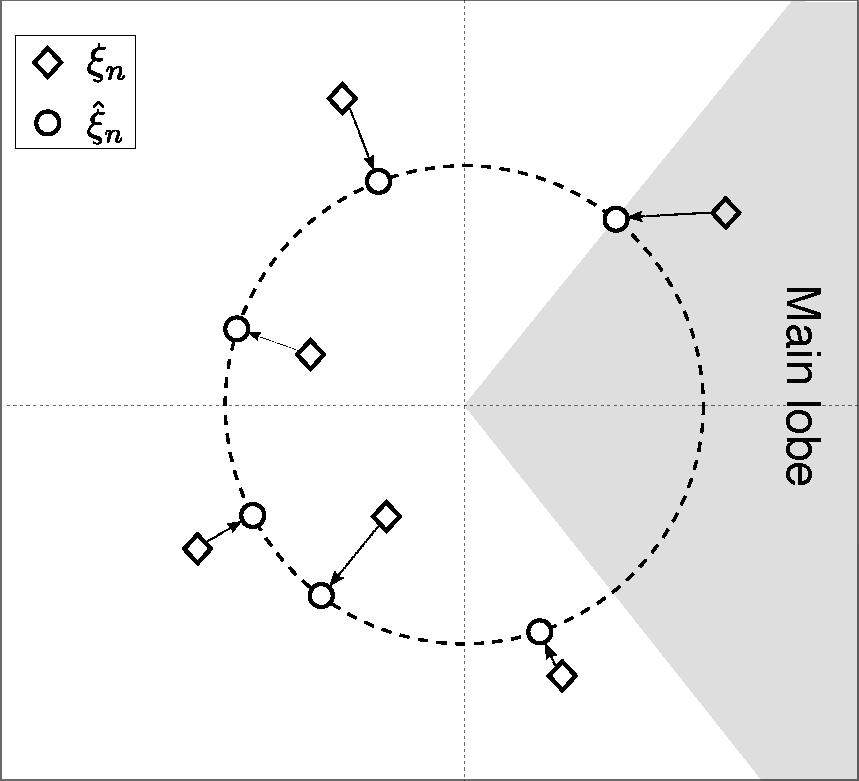
\includegraphics[width=0.9\textwidth]{ucmvdr_cartoon}  
\caption{Schematic shows the unit circle projection technique. The
  diamond markers denote the sample zeros ($\sampz_n$) and the circle
  markers denote the unit circle zeros ($\ucz$) obtained by radially
  projecting the sample zeros. The sample zeros within the main-lobe
  region ($-2/N \leq u \leq 2/N$) are moved to the closest CBF
  first-null location ($u_{\text{null}} = \pm 2/N$) on the unit circle.}
\label{fig:ucmvdr-cartoon}
\end{figure}

The projected unit circle zeros $\ucz_n$ are used to synthesize a unit
circle polynomial
\begin{align}
\label{eq:uc-poly}
\ucpoly(z) =& \prod\limits_{n=1}^{N-1}\frac{(1 - \ucz_n z\inv)}{(1 - \ucz_n)}. \nonumber \\
\intertext{Rewriting the polynomial in terms of the coefficients
}
\ucpoly(z) =& \sum\limits_{n=0}^{N-1} c_n^* z\inv.
\end{align}
Comparing \eqref{eq:uc-poly} to the definition of the array polynomial
\eqref{eq:beampat-poly}, the coefficients $c_n$s can be viewed as
beamformer weights. Thus, the UC MVDR ABF weight vector is defined as
$\wuc = [c_1, c_2, \ldots, c_N]\trans$. Evaluating $\ucpoly(z)$ on the
unit circle produces the UC MVDR ABF beampattern with $N-1$ nulls in
the directions corresponding to $\ucz_n$s and a unity gain in the look
direction ($\ulook = 0$), i.e., $\ucpoly(\expo{j\pi\ulook}) = 1$.

\begin{algorithm}
  \caption{DZ MVDR beamformer} \label{alg:ucmvdr}
  \begin{algorithmic}
    \Procedure{SMI MVDR}{$\datavec{}$}\Comment{Compute SMI MVDR weights}
     \State $\sampCov = \frac{1}{L}\sum\limits_{\ell=1}^L\datavec\datavec\herm$
     \State $\wsmi = {\sampCov\inv\replook}/{(\replook\herm\sampCov\inv\replook)}$
    \EndProcedure
    \Procedure{ProjectUnitCcircle}{$\wsmi$}\Comment{Project zeros to unit circle}
    \State $\smipoly(z) = \ztrans (\wsmi\herm) = G\prod\limits_{n=1}^{N-1}(1 - \sampz_nz\inv)$ 
    \State  $\sampz_n = r_ne^{j\omega_n}$ \Comment{SMI MVDR polynomial zero}
     \If{$|\omega_n| > 2\pi/N$}
     \State $\ucz_n = e^{j\omega_n}$     
     \ElsIf{$|\omega_n| \leq 2\pi/N$}
     \State $\ucz_n = e^{\sign(\omega_n){j2\pi/N}}$
     \EndIf
     \EndProcedure
     \Procedure{UC MVDR}{$\ucz_n$}\Comment{Compute UC MVDR weights}
    \State $\ucpoly(z) = \prod_{n=1}^{N-1}(1 - \ucz_n z\inv)/(1 - \ucz_n) = \sum_{n=0}^{N-1} c_n^*z^{-n}$ 
    \State $\wuc = [c_1, c_2,\ldots,c_N]\trans$
    \EndProcedure
  \end{algorithmic}
\end{algorithm}

%  In order to satisfy the
% distortionless constraint of the MVDR beamformer, the $c_n$s are
% scaled to force unity gain in the look direction. The resulting UC
% MVDR beamformer weight vector is
% $\wuc = {\bf{c}}/{\replook\herm\bf{c}}$ where
% $\mathbf{c} = [c_0, c_1 \ldots c_{N-1}]$ and $\replook$ is the array
% manifold vector for the look direction $\ulook = \cos(\theta_0)$.
% Since the polynomial zeros are invariant to coefficient scaling, the
% UC MVDR beampattern still has nulls in the same locations as the
% polynomial $\ucpoly(z)$.


\figurename{} \ref{fig:smi-ucmvdr-plots} shows a representative
example of the zero locations and the beampattern of a UC MVDR and the
SMI MVDR ABF using an $N = 11$ sensor ULA and $L = 12$ snapshots. Both
ABFs are steered to broadside ($\ulook = 0$) look direction and a
single interferer is present at $\uinter = \cos(\theta_I) = 3/N$. In
\figurename{}~\ref{fig:smi-ucmvdr-pzplot}, the green diamond markers
indicate the SMI MVDR polynomial zero locations and the red circle
markers indicate the UC MVDR zeros projected on unit
circle. \figurename{}~\ref{fig:smi-ucmvdr-bpplot} shows nulls and
lowered sidelobes in the UC MVDR beampattern (solid red) in contrast
to the shallow notches and higher sidelobes of the SMI MVDR
beampattern (dot-dash green). The lowering of the sidelobes reduces
the area under the beampattern magnitude, which in turn improves the
WNG of the UC MVDR as described by \eqref{eq:wng-beampat}.

As discussed in Sec.~\ref{sec:mvdr-poly}, the SMI MVDR polynomial
zeros are randomly perturbed in both magnitude and phase from the
ensemble zero locations on the unit circle. Projecting the SMI MVDR
polynomial zeros back on the unit circle corrects the magnitude
perturbation in the sample zeros thereby satisfying the
ensemble constraint of unit circle zeros. Moreover, the UC MVDR
weights can be seen as the closest approximation of SMI MVDR weights
in the ensemble constraint space, i.e., on the unit circle.

\begin{figure}[!hp]
\centering
\subfloat[Zero locations]
{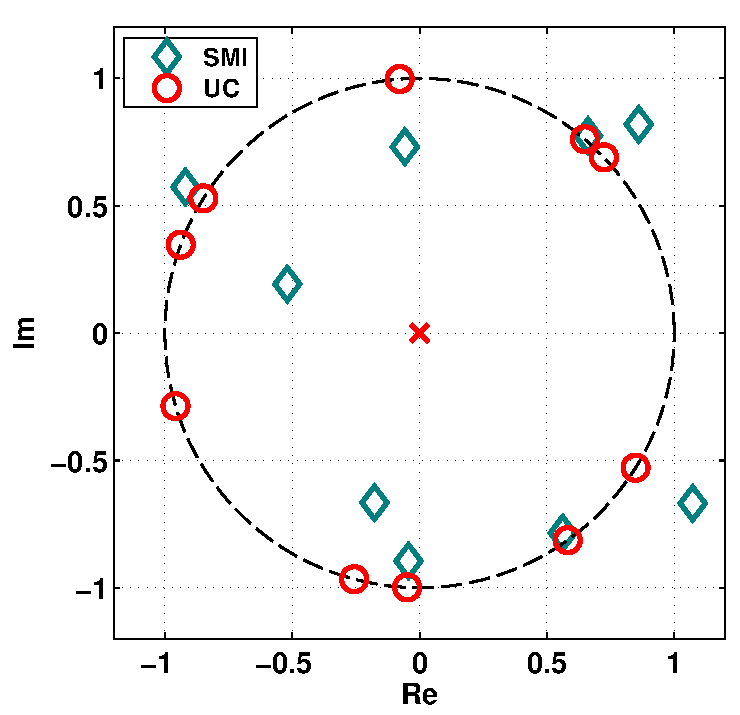
\includegraphics[width=3.5in]{mvdr_smi_dl_zfc_N11_pzplot_eg}  \label{fig:smi-ucmvdr-pzplot}}

\subfloat[Log-magnitude beampattern]{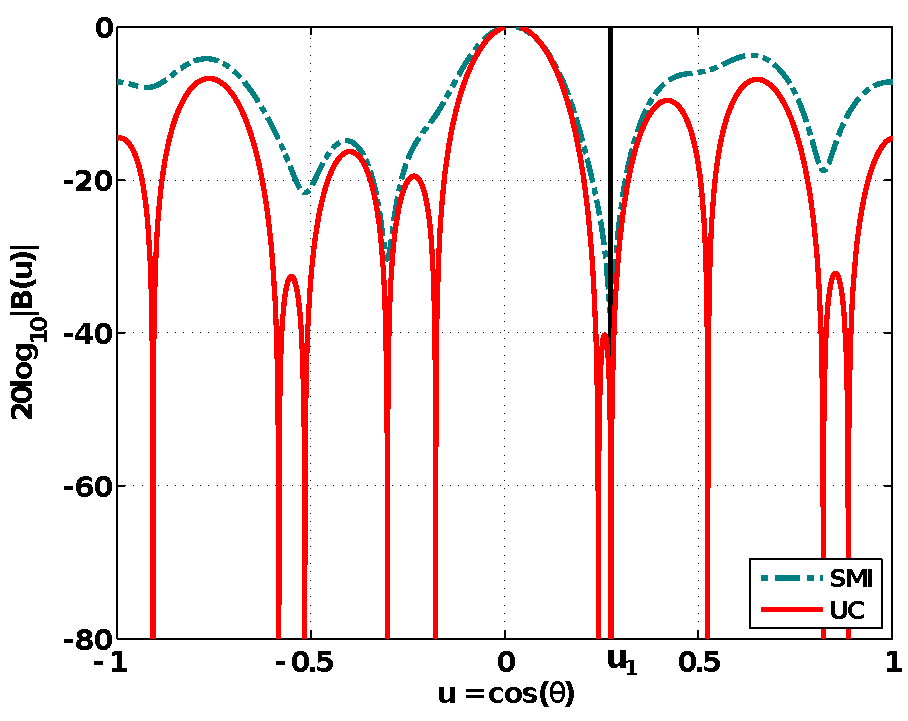
\includegraphics[width=3.5in]{mvdr_smi_dl_zfc_N11_bpplot_eg}  \label{fig:smi-ucmvdr-bpplot}}
\caption{Zero locations and log-magnitude beampatterns of a
  representative example of SMI MVDR (blue) and UC MVDR ABF (magenta)
  using $N = 11$ sensor ULA for $L = 12$ snapshots and look direction
  $\ulook = 0$. The unit circle zeros of the UC MVDR ABF produce nulls
  and lowers sidelobes compared to the SMI MVDR ABF beampattern.}
\label{fig:smi-ucmvdr-plots}
\end{figure}

%%% Local Variables: 
%%% mode: latex
%%% TeX-master: "main"
%%% End: 

\section{Simulation results}
\label{sec:ucbf-perf}
This section presents results of the simulation experiments evaluating
the performance of the UC MVDR ABF compared to the SMI MVDR and the DL
MVDR ABFs. All ABFs are implemented using $N = 11$ and $N = 51$
element ULAs and steered to the broadside look direction($\ulook =
0$). The experiments assume a passive sonar environment where the ABFs
often operate with barely sufficient snapshots $L = N + 1$ and two
snapshots per sensor $L = 2N$ is considered a snapshot rich scenario
\cite{cox2002adaptive,baggeroer1999passive}. The simulated snapshot
consists of a single loud interferer present at $\uinter = 3/N$ and a
unit power white background noise. For such measurement scenario, the
ABF output power $\pout$ is a sum of interferer contribution $\pinter$
and noise contribution $\pnoise$ as discussed in
\sect{}\ref{sec:output-power}. In the sequel, the two components of
the output power are referred to as the interferer output power
($\pinter$) and white noise output power
($\pnoise$). \sect{}\ref{sec:ucmvdr-interf-outp-result} compares the
interferer output power of the ABFs and
\sect{}\ref{sec:ucmvdr-wng-result} compares the WNGs of the
ABFs. Since the white noise output power is determined by the WNG, it
is sufficient to compare the WNGs of the ABFs. All the results are
averaged from a 3000 trial Monte Carlo experiment.

% The ABF output power is computed
% as $\pout = \wthat\herm \Cov \wthat$ where $\wthat$ is the ABF weight
% vector. Using the definition of the ECM for the single interferer case
% the output power is
% $\pout = \cov_I^2|\wthat\herm \rep_I|^2 + \cov_w^2||\wthat||^2 =
% \cov_I^2 \notchdepth + \cov_w^2 {\rm WNG}\inv = \pinter + \pnoise$.
% The total output power is the sum of interferer contribution
% ($\pinter$) and the white noise contribution ($\pnoise$).

%%% TODO
% JRB Comments
% Explain steps in order: first run UC MVDR trials, compute average WNG, then iterate estimating DL level for DL MVDR to match WNG.  Makes it clearer why you can't necessarily predict this.  

% We need to address Mestre DL algorithm at some point.  That really is the best existing benchmark, at least until Milutin Pajovic's papers are published.   

To ensure a fair comparison between the UC MVDR ABF and the DL MVDR
ABF, the DL level ($\dl$) can be chosen to match either the average
WNGs or the average notch depths (ND) between the two ABFs. In the
experiments, the DL level is chosen to match the average WNG between
the UC MVDR and the DL MVDR ABF. In order to determine the DL level,
the experiments first implement the UC MVDR for all trials and compute
the average WNG of the UC MVDR ABF. The DL level is then estimated
iteratively to match the average WNG between the UC MVDR and DL MVDR
ABFs.


\subsection{Interferer output power}
\label{sec:ucmvdr-interf-outp-result}
\figurename{}~\ref{fig:ecdf-plots} shows the empirical cumulative
distribution function (ECDF) of the interferer output power
($\pinter$) for the UC MVDR ABF compared to the SMI MVDR and DL MVDR
ABFs. The upper two panels show the ECDF graphs for the $N = 11$
sensor ULA and the lower two panels show the ECDF graphs for the $N =
51$ sensor ULA. The left two panels show the limited snapshot cases
where $L = N + 1$ and the right two panels show the snapshot rich case
where $L = 2N$. For all ULA sizes and snapshot cases, the sensor level
INR was set at $40$ dB. The dashed vertical line represents the
ensemble interferer output power $\pinter$ obtained from the MVDR
beamformer implemented using the ECM. The interferer output power
$\pinter$ corresponding to the ECDF equal to $0.5$ defines the median
value. The closer the median of the interferer output power $\pinter$
of the ABFs is to the dashed vertical line, higher the better the
probability of producing output comparable to the ensemble case. For
all four cases examined, the DL level for the DL MVDR ABF is chosen to
match the average WNGs as described earlier.

Over the observed interferer output power range in
\figurename{}~\ref{fig:ecdf-plots}, the UC MVDR ABF exhibits
higher probability of achieving lower interferer output power
$\pinter$ compared
against both SMI MVDR and DL MVDR ABFs. For instance in
\figurename{}~\ref{fig:ecdf_N11L12INR40} the median output power of UC
MVDR was approximately 20 times lower than SMI MVDR and 10 times lower
than DL MVDR ABF. The DL MVDR has improved interferer
suppression over SMI MVDR as expected, but UC MVDR has improved
performance compared to both SMI MVDR and DL MVDR ABFs.

\begin{figure}[!hp]
  \centering
  \subfloat[N = 11, L = 12]{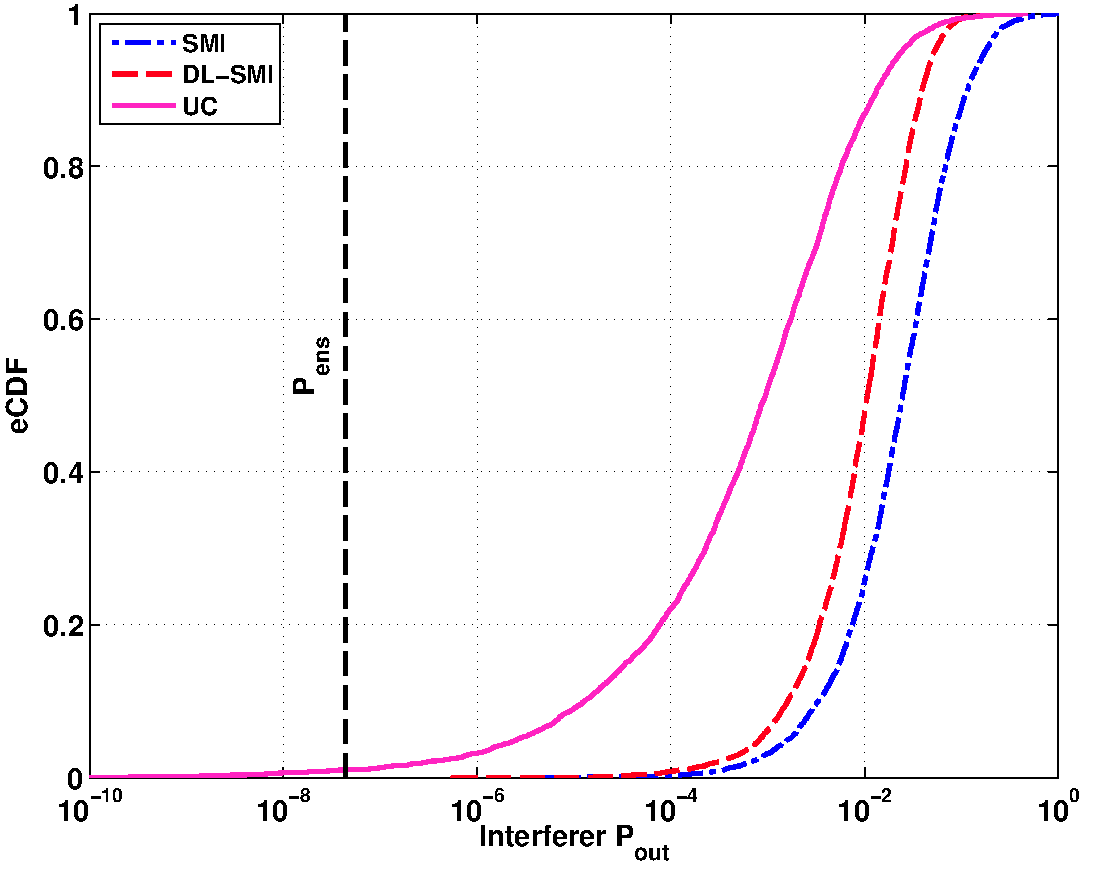
\includegraphics[width=3in]{mvdr_smi_zfc_dl_Po_ecdf_N11L12_INR40}%
    \label{fig:ecdf_N11L12INR40}}
  \subfloat[N = 11, L = 22]{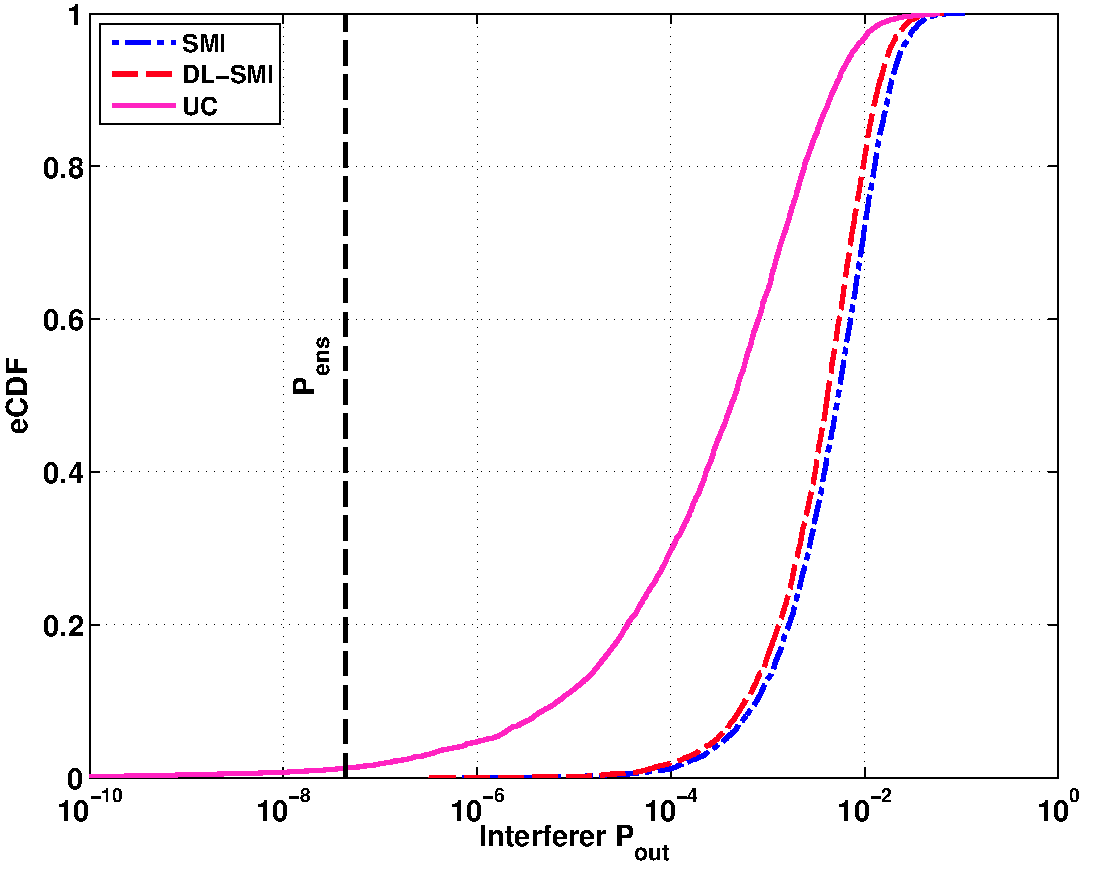
\includegraphics[width=3in]{mvdr_smi_zfc_dl_Po_ecdf_N11L22_INR40}%
    \label{fig:ecdf_N11L22INR40}}\\
  \vfill
  \subfloat[N = 51, L = 52]{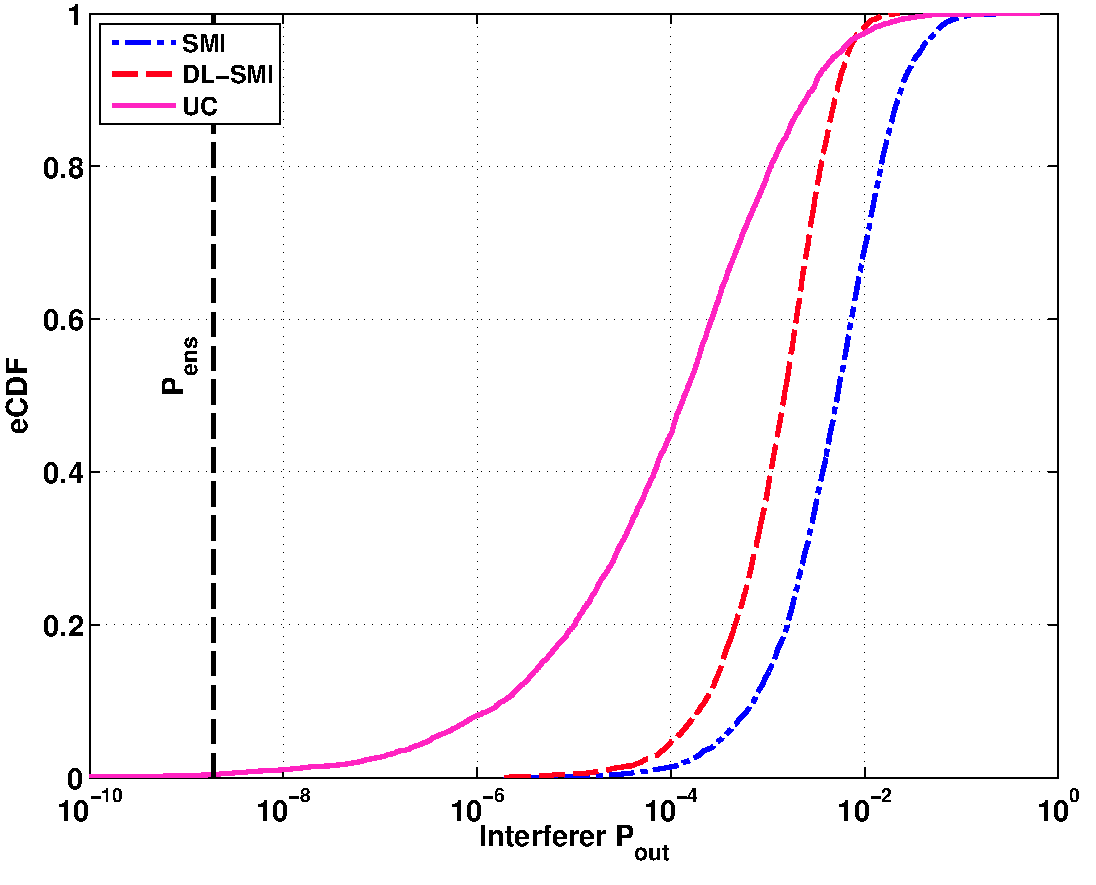
\includegraphics[width=3in]{mvdr_smi_zfc_dl_Po_ecdf_N51L52_INR40}%
    \label{fig:ecdf_N51L52INR40}}
  \subfloat[N = 51, L = 102]{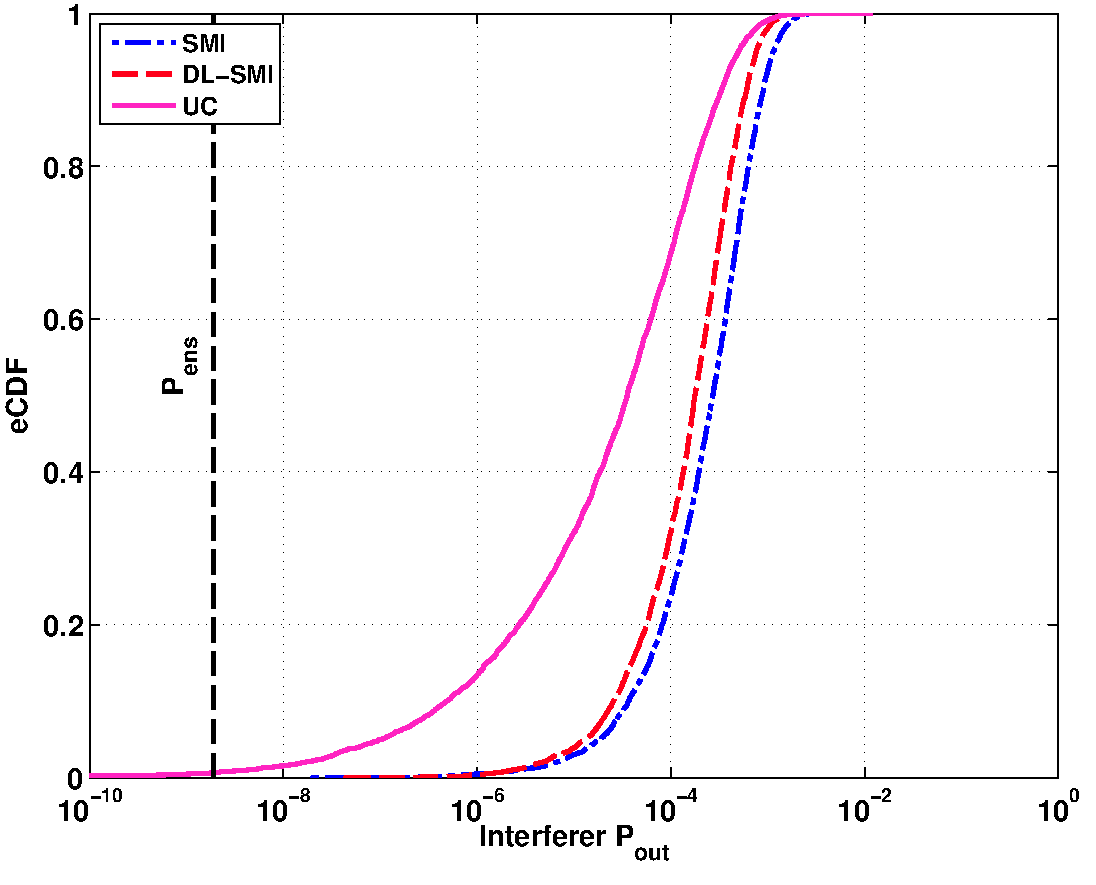
\includegraphics[width=3in]{mvdr_smi_zfc_dl_Po_ecdf_N51L102_INR40}%
    \label{fig:ecdf_N51L102INR40}}
  \caption[Comparison of the ECDF of the interferer contributed output
  power.]{ ECDF of the interferer contributed output power
    $\pinter$. The ECDFs are compared between the SMI MVDR, DL MVDR
    and the UC MVDR ABFs. The ABFs use $N = 11$ element ULA in the top
    panel and $N = 51$ element ULAs in the bottom panel. The left
    panels shows the snapshot deficient case ($L = N + 1$) and the
    right panels shows the snapshot rich case ($L = 2N$). In each
    panel the dashed vertical line denotes the interferer contributed
    output power for the ensemble MVDR ABF. In all cases, the UC MVDR
    ABF suppresses the interferer better compared to the SMI MVDR and
    DL MVDR ABFs.}
  \label{fig:ecdf-plots}
\end{figure}

\figurename{}~\ref{fig:pout-mean-var-plots} compares the squared mean
(solid) and variance (dashed) of interferer output power $\pinter$ for
UC MVDR and SMI MVDR ABFs over a range of INR values from 0 dB to 40
dB. The interferer output power $\pinter$ of the UC MVDR ABF has lower
mean and variance compared to the interferer output power $\pinter$ of
the SMI MVDR ABF. The reduced mean interferer output power $\pinter$
using UC MVDR supports the earlier conclusion that UC MVDR ABF
provides improved interferer suppression. The reduced variance on
interferer output power suggests the UC MVDR ABF should achieve better
detection performance as well.

\begin{figure*}[!hp]
  \centering
  \subfloat[L = 12 snapshots]
{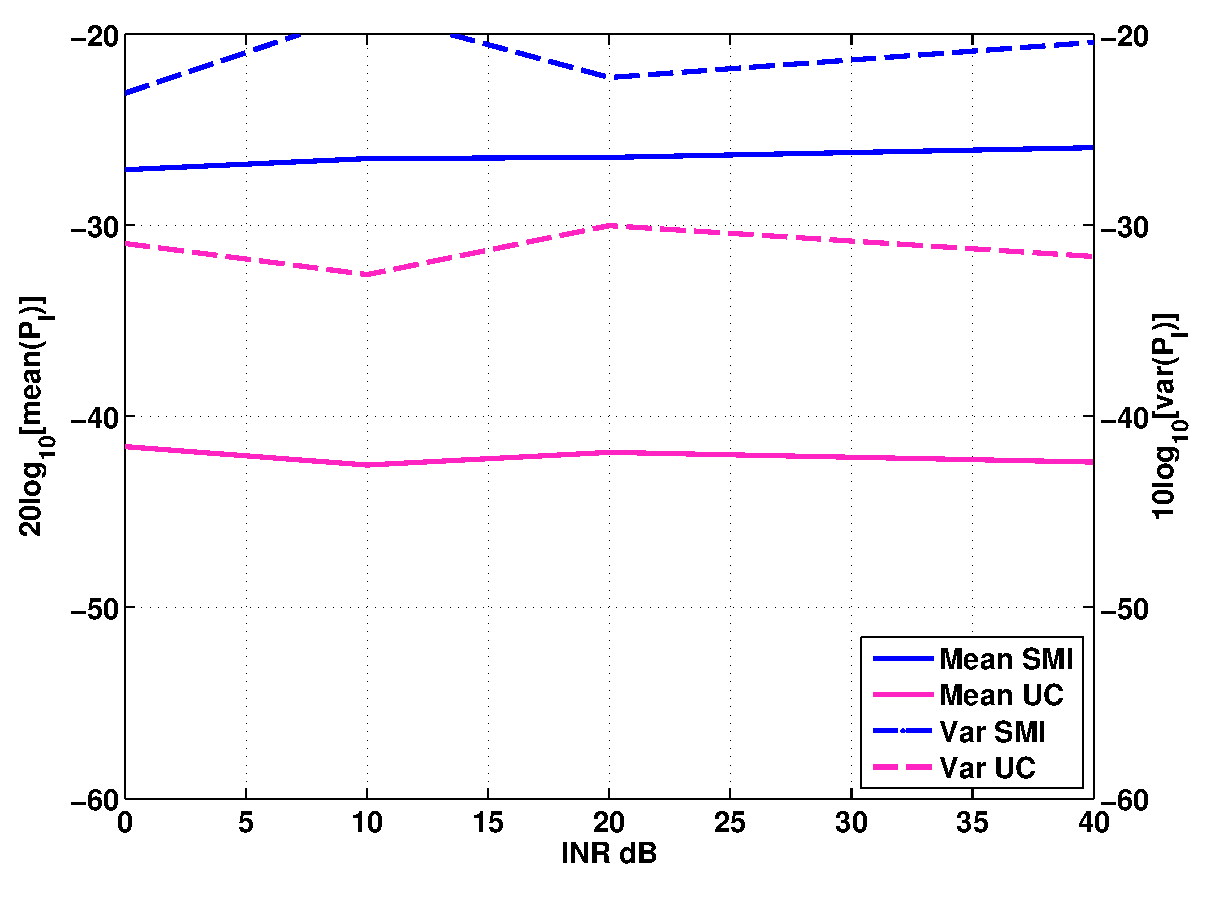
\includegraphics[width=4in]{mvdr_smi_zfc_Po_meansq_var_N11_L12}%
    \label{fig:mpout_N11L12}}  \hfill
  \subfloat[L = 22 snapshots]
{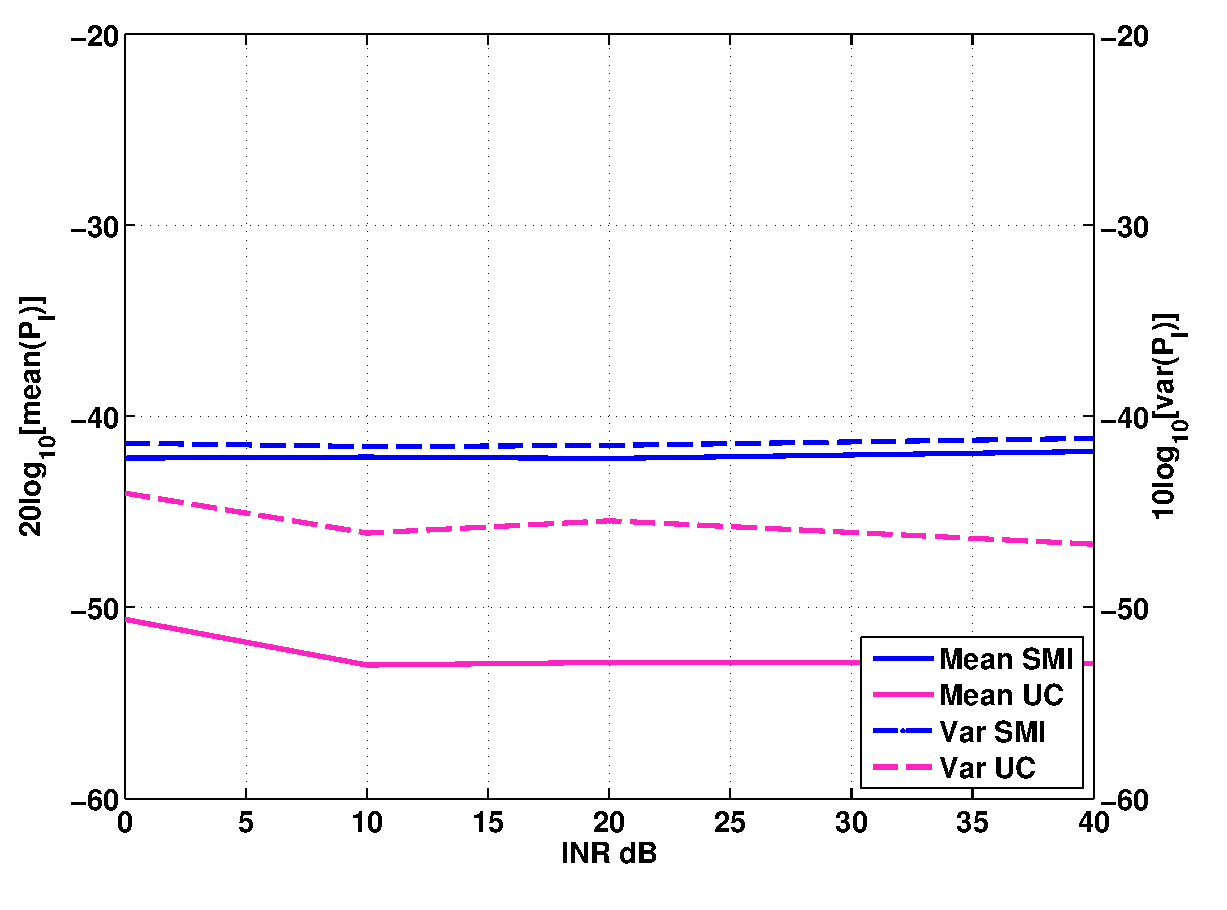
\includegraphics[width=4in]{mvdr_smi_zfc_Po_meansq_var_N11_L22}%
    \label{fig:mpout_N11L22}}
  \caption{Dual y-axis plot of mean and variance of interferer output power $\pinter$ for the SMI MVDR (blue) and the UC MVDR ABF (magenta). Both ABFs are implement using $N = 11$ element ULA and SCM computed from $L = 12$ snapshots in top panel and $L = 22$ snapshots in bottom panel. The UC MVDR ABF yields interferer contributed output power with lower mean and variance compared to the SMI MVDR ABF.}
  \label{fig:pout-mean-var-plots}
\end{figure*}

\subsection{White noise gain}
\label{sec:ucmvdr-wng-result}
\figurename{}~\ref{fig:wng} compares the WNG of the UC MVDR and the
SMI MVDR ABF implemented using $N = 11$ sensor ULA and $L = 12$
snapshots. The maximum WNG for this experiment is $N = 11$ and
corresponds to the CBF
\cite{vtree2002oap}. \figurename{}~\ref{fig:wng-hist-plot} compares
the histograms of the WNG for the UC MVDR and SMI MVDR ABFs. The UC
MVDR ABF achieves improved WNG compared to the SMI MVDR ABF. The
dashed vertical line denotes the ensemble WNG of $10.473$. The UC MVDR
ABF has a greater probability of achieving higher WNG with an average
WNG of $5.672$ compared to an average WNG of $2.629$ using the SMI
MVDR ABF.

\figurename{}~\ref{fig:wng-scatter-plot} is a scatter plot of the WNG
for the UC MVDR and the WNG for the SMI MVDR ABF. Each point in the
scatter plots the WNG of the UC MVDR ABF against the WNG of SMI MVDR
ABF for a single realization of the ABFs in the Monte Carlo
experiment. The scatter plot shows that the UC MVDR has a higher WNG
than SMI MVDR ABF in each trial instance except for small number of
cases (bottom left corner in \figurename{}~\ref{fig:wng-scatter-plot})
where both ABFs have low WNG. Similar results were observed for the
case of $N = 51$ sensor ULA. Thus, on average the UC MVDR ABF has a
higher WNG than the SMI MVDR ABF. In addition of being able to
suppress white noise, the improved WNG implies that the UC MVDR ABF is
also less sensitive to array parameter perturbations
\cite{Gilbert1955,vtree2002oap}.

% Although a DL MVDR is able to achieve a
% specified WNG with a choice of DL level, it requires
% numerically solving for the DL level \emph{a priori} where as UC MVDR improves the
% WNG devoid of such \emph{a priori} requirements.

\begin{figure}[!hp]
  \centering
  \subfloat[]{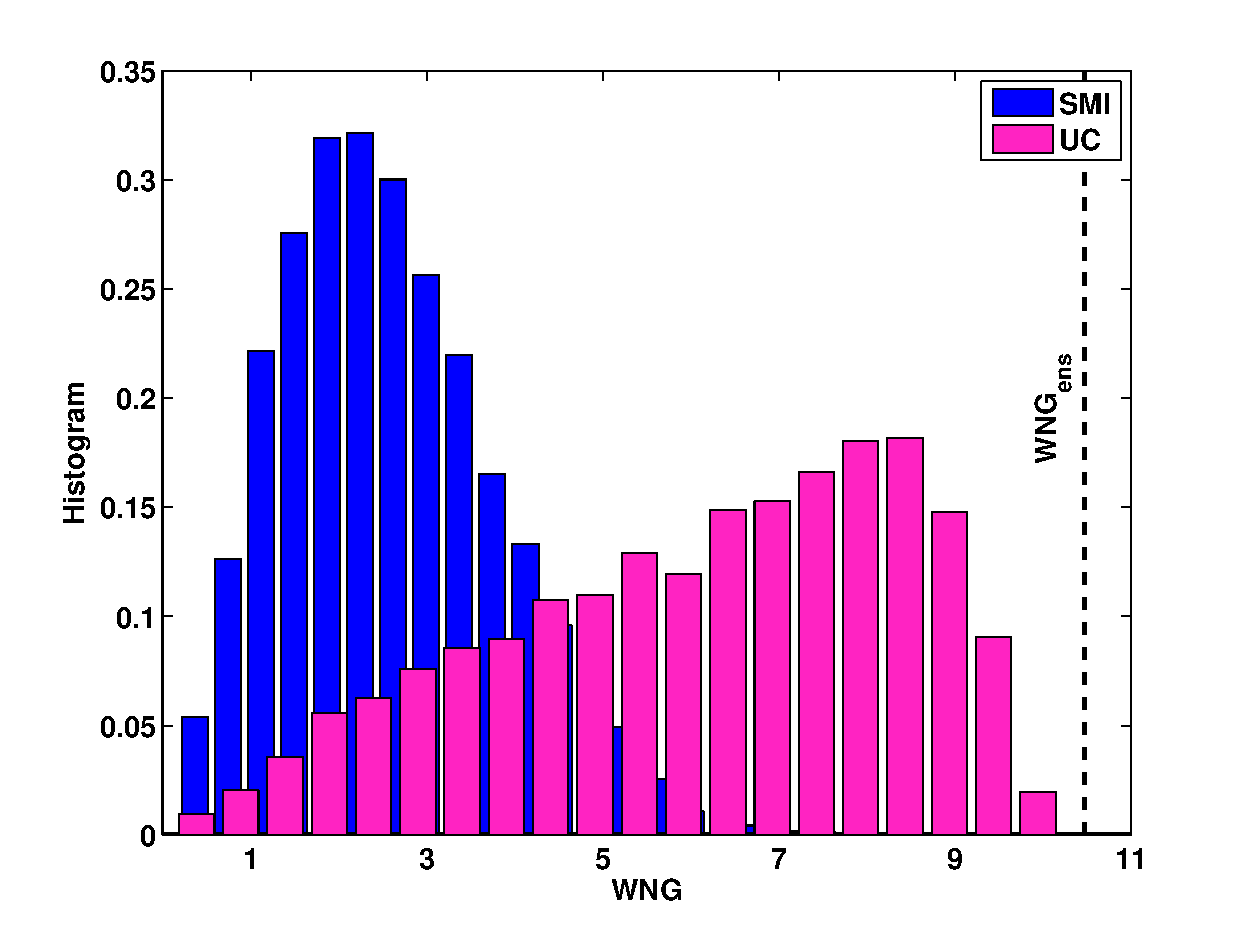
\includegraphics[width=3.5in]{mvdr_smi_zfc_WNG_hist_N11L12_INR40}
    \label{fig:wng-hist-plot}}

\subfloat[]{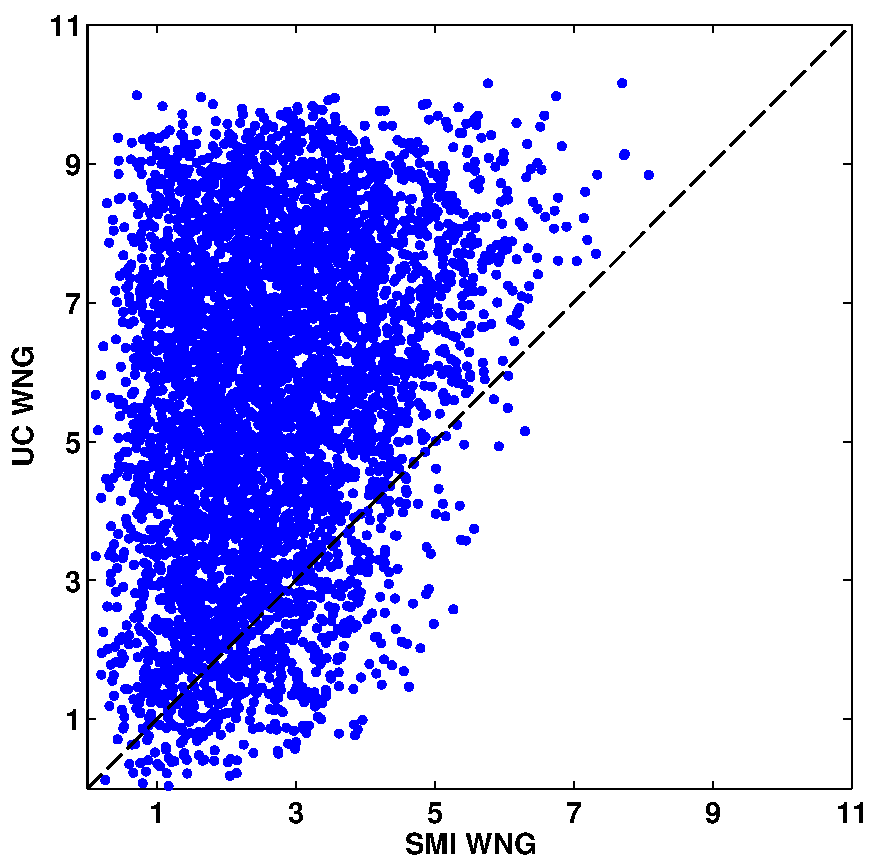
\includegraphics[width=3in]{mvdr_smi_zfc_WNG_scatter_N11L12_INR40}
    \label{fig:wng-scatter-plot}}
  \caption{Comparison of WNG between the UC MVDR and the SMI MVDR ABF,
    both implemented using an $N = 11$ element ULA and $L = 12$
    snapshots. Top panel compares the histogram of WNGs and the lower
    panel is a scatter plot of the WNGs. On average, the UC MVDR ABF
    has higher WNG compared to the SMI MVDR ABF. }
  \label{fig:wng}
\end{figure}

\subsection{UC MVDR and DL MVDR polynomial zeros}
\label{sec:ucmvdr-dlmvdr}
The UC MVDR and the DL MVDR ABF are both derived by modifying the SMI
MVDR ABF. As described above, the UC MVDR ABF moves the sample zeros
radially back on to the unit circle. This section discusses how DL
changes the DL MVDR zeros and compares with the UC MVDR polynomial
zeros.

\figurename{}~\ref{fig:ucbf-dlsmi-pzplot} shows array polynomial zeros
a representative example of ABFs implemented using an $N = 11$ element
ULA and steered to $\ulook = 0$. A single interferer is present at
$\uinter = 3/N$ denoted by the radial dashed line. The blue squares
denote the sample zeros, the magenta circles denote the UC MVDR zeros
and the black diamonds denote the CBF zeros. Each black dot denotes a
DL MVDR zero location as the DL level changes from $-40$ dB to $40$ dB
in $4$ dB steps. When the DL level $\dl \approx 0$, the DL MVDR zeros
are essentially in sample zero locations. As the DL level increases,
the DL MVDR zeros converge towards the CBF zero locations as denoted
by the intermediate dot markers. The intermediate dot markers trace a
trajectory of DL MVDR zero locations starting from the sample zero
location to CBF zero location, as the DL level changes. A specific
trajectory is associated with each sample zero. Hence, changing the DL
level moves the DL MVDR zeros along specific trajectories. As
previously seen in \sect{}\ref{sec:diagonal-loading}, Mestre and
Lagunas present an approach to compute the optimal DL level
\cite{mestre2006finite}. The DL MVDR zeros associated with the optimal
DL level are constrained on the specific trajectories of each sample
zero, and may not be particularly close to the ensemble zero
locations. In fact, any choice of DL level always yields zeros along
the trajectories from sample zero to CBF zero
locations. Comparatively, the UC MVDR ABF approach of moving the
sample zeros radially back to the unit circle is markedly different
approach.

Moreover, one use of applying DL is to improve WNG of the ABFs
\cite{vtree2002oap}. As the DL MVDR zeros move closer to the CBF zero
locations, the WNG performance improves. However, moving zeros closer
to the CBF zero locations leads to loss of ND in the interferer
direction. Hence choosing DL level involves a trade off between loss of
interferer suppression and improved WNG. On the contrary, the unit
circle zeros of the UC MVDR create beampattern nulls which
simultaneously improve notch depth and lower sidelobes. Consequently,
the UC MVDR ABF improves both the interferer suppression and the WNG
performance as discussed in \sect{}\ref{sec:ucbf-perf}. Further, the
UC MVDR ABF does not require choosing a tuning parameter like the DL
level.

% The optimal DL level computed using Mestre and Lagunas
% \cite{mestre2006finite} approach chooses where to stop along the
% trajectory but the trajectories move
% the zeros towards the CBF zero locations instead of the ensemble zero
% locations. The DL MVDR zeros may not be particularly close to the
% ensemble zero locations.  The UC MVDR zeros do not follow the DL MVDR
% zeros trajectory and as seen above improve both WNG and interferer
% suppression.
 

% One benefit of applying DL is that it improves the WNG of the SMI MVDR
% ABF \cite{Gilbert1955}. This improvement in the WNG lowers the
% beampattern sidelobes of the ABF as mentioned earlier in
% \sect{}\ref{sec:wng}. \figurename{}~\ref{fig:ucbf-dlsmi-pzplot} shows
% that the DL MVDR ABF is able to lower the sidelobes by moving the
% polynomial zeros closer to the unit circle. As the zeros move closer
% to the unit circle, the beampattern local minimas become deeper and
% pull down the sidelobes. In contrast, the UC MVDR ABF always projects
% the SMI MVDR polynomial zeros to the unit circle. The unit circle
% zeros ensure nulls in the beampattern and also reduce sidelobes
% improving WNG. Moreover, as discussed earlier the UC MVDR ABF does not
% require an \emph{a priori} choice of a tuning parameter like the DL
% level.

\begin{figure}[!hp]
  \centering
  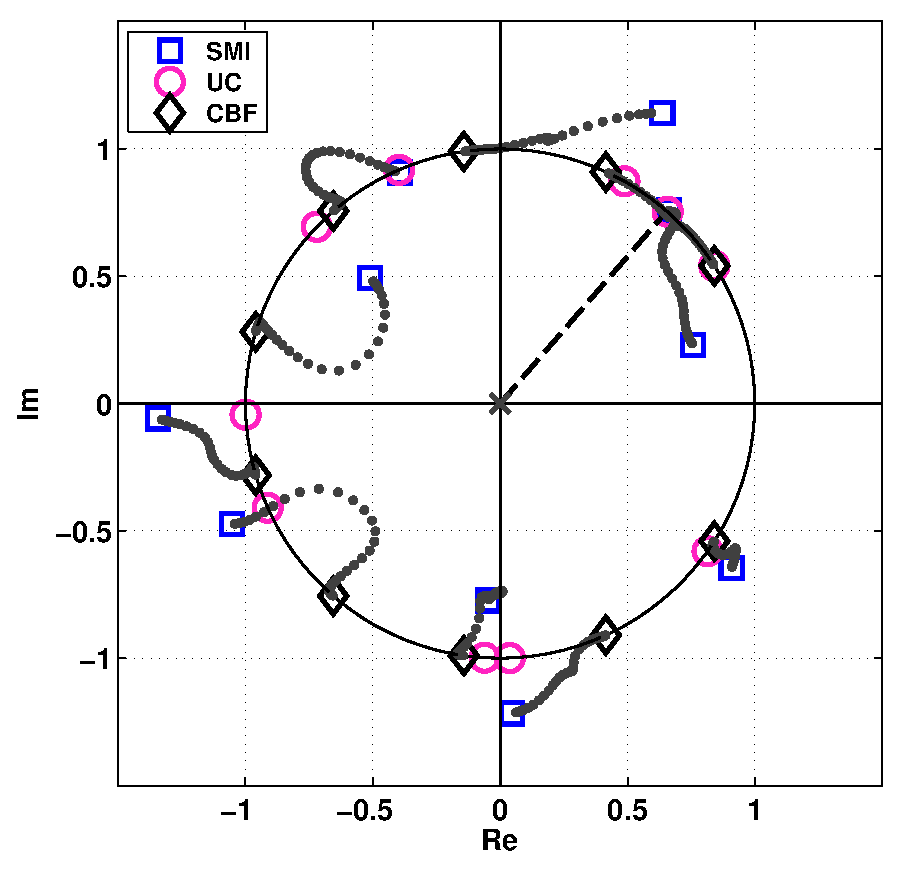
\includegraphics[width=\textwidth]{mvdr_smi_uc_cbf_dl_varying_pzplot}
  \caption{UC MVDR polynomial zeros compared against DL MVDR
    polynomial zeros as the DL level $\dl$ is increased from $-40$ dB to
    $40$ dB. The DL MVDR polynomial zeros asymptotically converge to CBF polynomial zero locations as $\dl \rightarrow \infty$. }
  \label{fig:ucbf-dlsmi-pzplot}
\end{figure}

%%% Local Variables: 
%%% mode: latex
%%% TeX-master: "main"
%%% End: 

% --------------------
% ====================

\section{UC MVDR ABF in snapshot deficient case}
\label{sec:uc-mvdr-snapshot-def}
This section presents one approach to implement the UC MVDR ABF in a
snapshot deficient scenario ($L < N$). The UC MVDR algorithm begins by
initially computing the SMI MVDR weights. However, when snapshot
deficient the SCM is not invertible and hence SMI MVDR ABF cannot be
directly implemented as mentioned in Ch.~\ref{ch:lit-rev}. One common
solution is to apply diagonal loading (DL) to the SCM to make it full
rank and hence invertible. The SMI MVDR weights are then computed
using the full rank DL SCM. The DL level can be chosen using one of the
approaches mentioned in \sect{}\ref{sec:ucbf-perf}. The previous
section discussed the effect of applying DL on the locations of the
sample zeros. When the DL level is small enough the
effect on the SMI MVDR polynomial zero locations is negligible.

In the snapshot deficient scenario, an alternative approach is to
choose a minimal DL level $\dlmin$ just enough to make the SCM
invertible and compute the SMI MVDR weights. The SMI MVDR weights
evaluated using the minimally loaded SCM can be seen as the closest
approximation to the SMI MVDR weights when just enough snapshots are
available ($L \approx N$) to obtain a full rank SCM without having to
apply DL. Following this alternative approach, the proposed
implementation of the UC MVDR ABF in snapshot deficient case begins
with a minimally loaded SCM used to compute the SMI MVDR
ABF. Subsequently the UC MVDR ABF weights are derived by projecting
the sample zeros onto the unit circle as described
previously.

\figurename{}~\ref{fig:ucmvdr-snapshot-deficient} evaluates the UC
MVDR ABF implemented for a $N = 11$ sensor ULA in two snapshot
deficient cases. The top panel corresponds to the case with $L = 10$
snapshots and the bottom panel corresponds to the case with $L = 5$
snapshots. In both panels, the solid magenta curve shows the
interferer output power ECDF graph for the UC MVDR ABF implemented
using a minimal DL level \mbox{$\dl_{min} = 10^{-8}$}. The dot-dashed
red curve shows the interferer output power ECDF graph for the DL MVDR
ABF. The DL level $\dl$ is chosen to match the average WNG with the UC
MVDR ABF. As described in \sect{}~\ref{sec:ucbf-perf}, finding the DL
level for the DL MVDR ABF involves first implementing the UC MVDR ABF
with minimal DL for all trials and computing the average WNG. The DL
level for DL MVDR is estimated iteratively to match average WNG
between the two ABFs. Following this approach, in the top panel use
$\dl = 0.1080$ and in the bottom panel uses $\dl = 0.5856$ for the DL
MVDR ABF. Comparison of the ECDF graphs show that in both snapshot
cases, the UC MVDR ABF exhibits higher probability of suppressing the
interferer compared to the DL MVDR ABF. This implies even in a
snapshot deficient case, on average the UC MVDR ABF implemented using
the minimal DL approach attenuates interferer better than the DL MVDR
ABF.

\begin{figure*}[!hp]
  \centering
  \subfloat[L = 10, $\dl = 0.1080$]
  {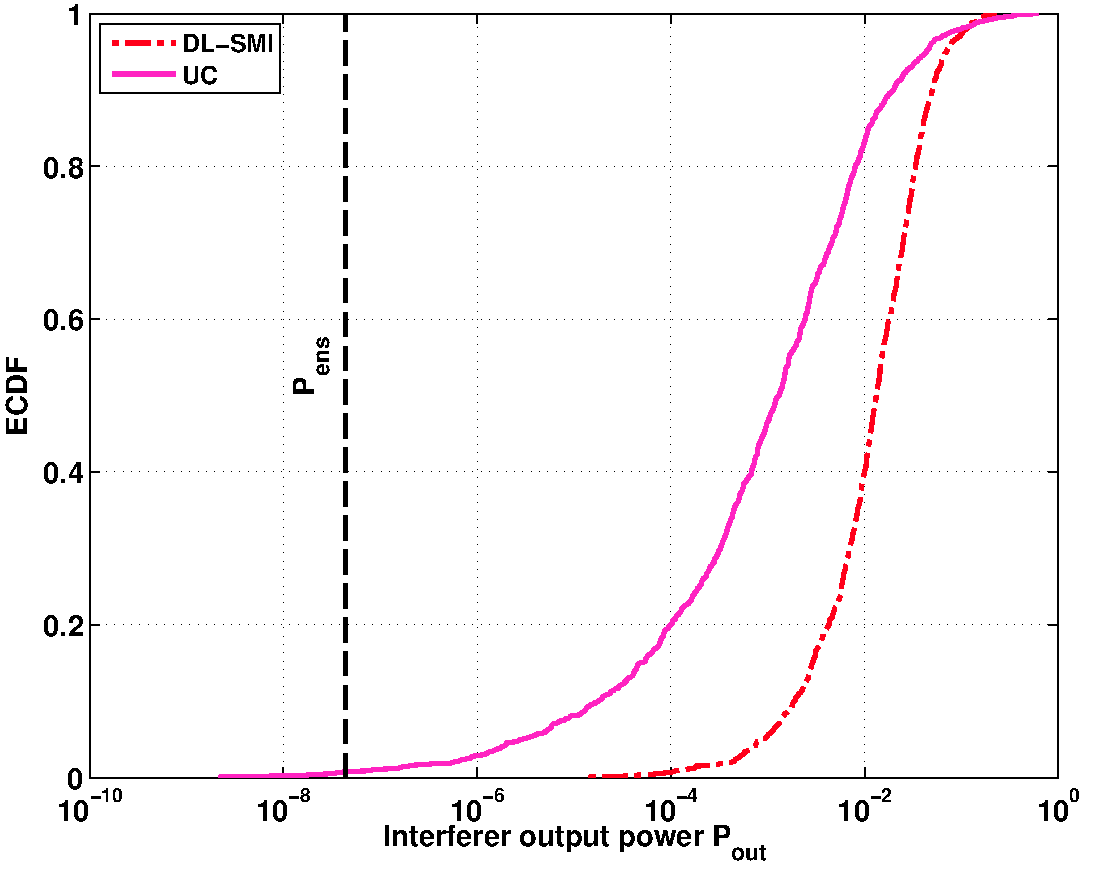
\includegraphics[width=3.5in]{mvdr_dlsmi_uc_ssd_Po_ecdf_N11L10_INR40.pdf}}  

  \subfloat[L = 5, $\dl = 0.5856$]
  {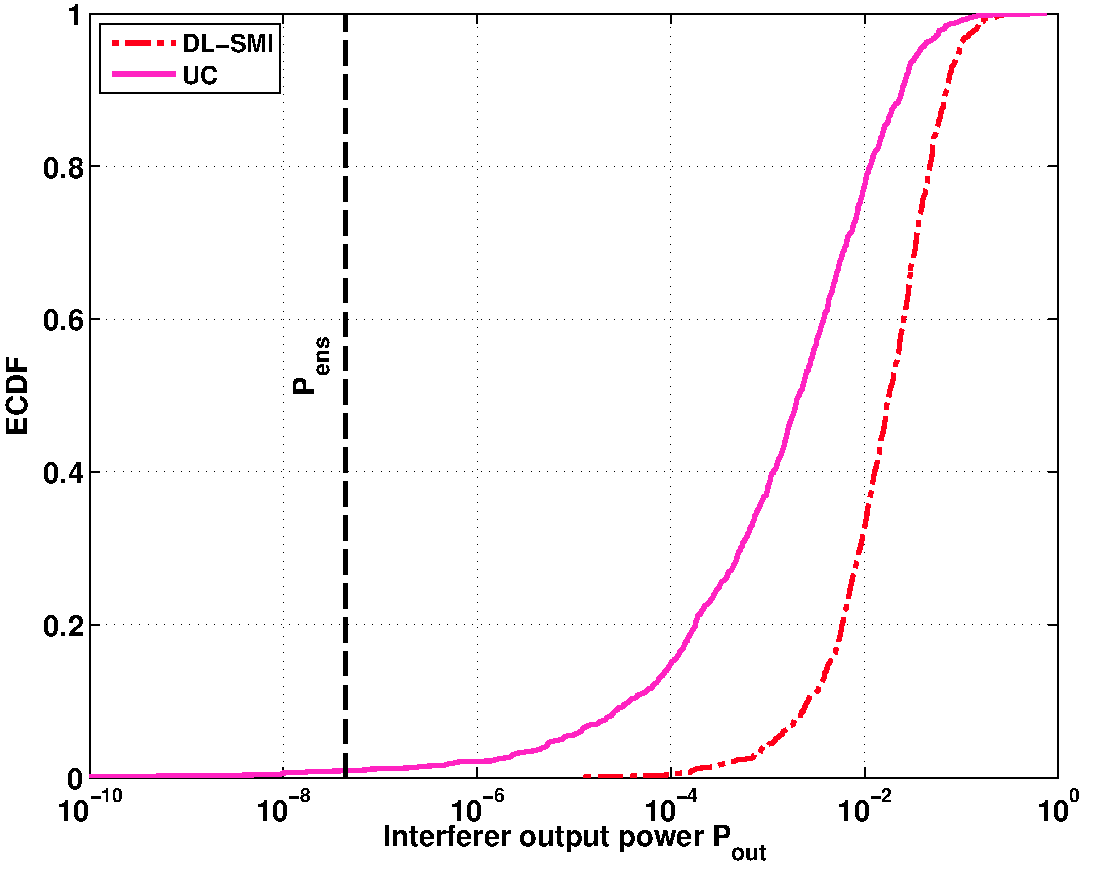
\includegraphics[width=3.5in]{mvdr_dlsmi_uc_ssd_Po_ecdf_N11L5_INR40.pdf}}

  \caption[ECDF of interferer contributed power for the UC MVDR ABF
  and the DL MVDR ABF in a snapshot deficient scenario.]{ECDF of
    interferer contributed output power compared between the UC MVDR
    ABF and the DL MVDR ABF in a snapshot deficient scenario. Both
    ABFs are implemented using $N = 11$ element ULA and the top panel
    considers $L = 10$ snapshots while the bottom panel considers
    $L = 5$ snapshots available to compute SCM. In both cases, the UC
    MVDR ABF uses a minimal DL ($\dl_{min} = 1e^{-8}$) and the DL MVDR
    ABF uses a DL level set to match the WNG with the UC MVDR ABF. The
    UC MVDR }
  \label{fig:ucmvdr-snapshot-deficient}
\end{figure*}

\section{ Unit Circle DMR ABF}
\label{sec:uc-mvdr-dmr}
As previously noted, the DMR ABF is another practical implementation
of the MVDR beamformer. The DMR ABF is almost always implemented using
the SCM. The DMR ABF replaces the SCM in \eqref{eq:mvdr-wt} with the
structured DMR SCM \eqref{eq:dmr-scm} to compute the DMR ABF
weights. The ensemble form of the DMR ABF is essentially the MVDR
beamformer in white background noise. Following a
similar approach as the UC MVDR ABF, a unit circle DMR (UC DMR) ABF is
derived by projecting the DMR polynomial zeros on the unit circle. The
difference from the UC MVDR ABF is that the SCM noise eigenvalues are
averaged implementing the unit circle constraint.
  
\figurename{}~\ref{fig:uc-mvdr-dmr-pout} compares the interferer
output power ECDF of the UC DMR ABF, the UC MVDR and the SMI MVDR
ABF. The ABFs are implemented using $N = 11$ sensor ULA and $L = 12$
snapshots. A single interferer with $40$ dB INR is present at
direction $\uinter = 3/N$. Knowing that only a single interferer is
present, the dominant subspace dimension for the DMR SCM equals to
one. The noise eigenvalue of the DMR SCM is averaged from the $10$
smallest eigenvalues of the SCM. In
\figurename{}\ref{fig:uc-mvdr-dmr-pout}, the top panel compares the
ECDF graphs of the UC MVDR, the UC DMR and the SMI MVDR
ABFs. Comparisons of the output power ECDF graphs show that the UC
MVDR ABF and the UC DMR ABF have comparable ability to suppress
interferer. As expected both the UC MVDR and the UC DMR ABFs perform
better than the SMI MVDR ABF. The bottom panel shows a scatter plot
where each dot marker denotes the WNG of the UC MVDR ABF against the
WNG of the UC DMR ABF. Examining the WNG scatter plot, the WNG of the
UC MVDR ABF is almost always lower than the WNG of the UC DMR ABF. The
WNG of the UC MVDR ABF exhibits high variability while the WNG of the
UC DMR ABF has almost no variability and on average comparable to the
optimal WNG of $N = 11$. Wage and Buck have shown that in case of a
signal strong interferer outside the main-lobe, the WNG of the DMR ABF
has low variability and on average the WNG is close to the optimal WNG
of $N$\cite{wage2013dmr}. The UC DMR ABF inherits the WNG behavior of
the DMR ABF. These results indicate that compared to the UC MVDR ABF,
the UC DMR ABF exhibits similar ability to suppress the interferer
and a better WNG performance. However, the UC DMR ABF is limited by
the need to determine the dominant subspace dimension before
implementing the ABF whereas the UC MVDR ABF is devoid of such prior
requirements.

\begin{figure}[!hp]
  \centering
  \centering
  \subfloat[]
  {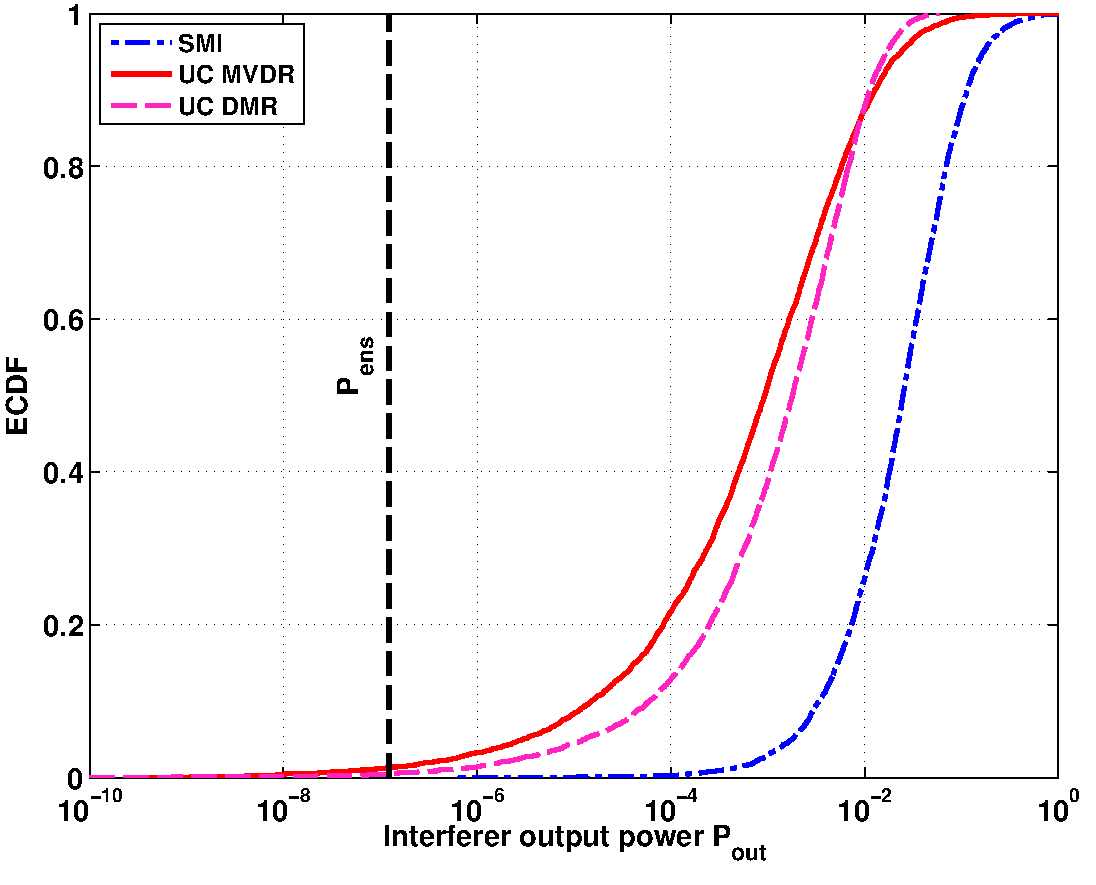
\includegraphics[width=3.5in]{smi_ucmvdr_ucdmr_Po_ecdf_N11L12_INR40.pdf}}  

  \subfloat[]
  {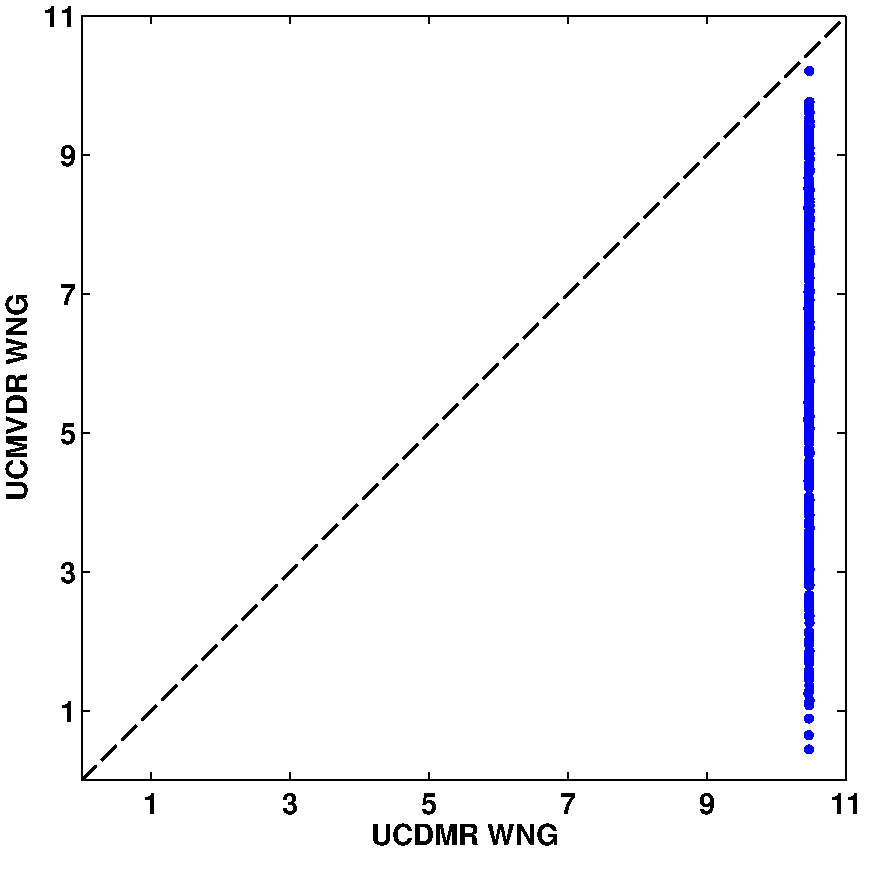
\includegraphics[width=3in]{smi_ucmvdr_ucdmr_WNG_scatter_N11L12_INR40.pdf}}
  \caption[Output power comparison between UC MVDR and UC DMR]{(a)
    ECDF of the interferer contributed output power compared between
    the UC MVDR, UC DMR and the SMI MVDR ABFs. (b) Scatter plot of the
    WNGs of the UC MVDR and UC DMR ABFs. All ABFs are implemented
    using $N = 11$ sensor ULA and $L = 12$ snapshots. The UC DMR attenuates interferer similarly to the UC MVDR ABF and has superior WNG.}
  \label{fig:uc-mvdr-dmr-pout}
\end{figure}

\section{Summary}
\label{sec:ch3-summary}
This chapter presents the UC MVDR ABF which projects the SMI MVDR
polynomial zeros radially on the unit circle to create perfect nulls
in the beampattern. By moving the sample zeros to the
unit circle, the UC MVDR zeros satisfy the unit circle constraint on
the ensemble zeros and creates deeper beampattern notches in the
interferer directions. In a snapshot deficient scenario the UC MVDR
ABF is derived from a SMI MVDR ABF evaluated using a minimally loaded
SCM. Numerical simulations show that the UC MVDR ABF suppresses
interferer better than both the SMI MVDR and DL MVDR ABF. Comparing
the WNG of the ABFs shows that on average the UC MVDR ABF has
higher a WNG than the SMI MVDR. Also, the UC MVDR ABF interferer
suppression is comparable to the UC DMR ABF. However unlike the DL MVDR ABF and the UC DMR ABF both of which requires choosing a design parameter,
the UC MVDR is not constrained to such requirements.
%%% Local Variables:
%%% TeX-master: "main"
%%% End: